
%%%%%%%%%%%%%%%%%%%%%%%%%%%%%%%%%%%%%%%%%%%%%%%%%%%%%%%%%%%%%%%%%%%%%%%%%%%%%%%%%%%%%%%
%%%%%%%%%%%%%%%%%%%%%%%%%%%%%%%%%%%%%%%%%%%%%%%%%%%%%%%%%%%%%%%%%%%%%%%%%%%%%%%%%%%%%%%
% 
% This top part of the document is called the 'preamble'.  Modify it with caution!
%
% The real document starts below where it says 'The main document starts here'.

\documentclass[12pt]{article}

\usepackage{amssymb,amsmath,amsthm}
\usepackage[top=1in, bottom=1in, left=1.25in, right=1.25in]{geometry}
\usepackage{fancyhdr}
\usepackage{enumerate}
\usepackage{listings}
\usepackage{graphicx}
\usepackage{float}
\usepackage{multicol}
% Comment the following line to use TeX's default font of Computer Modern.
\usepackage{times,txfonts}
\usepackage{mwe}
\usepackage{caption}
\usepackage{subcaption}
\usepackage{svg}





\makeatletter
\renewcommand*\env@matrix[1][*\c@MaxMatrixCols c]{%
  \hskip -\arraycolsep
  \let\@ifnextchar\new@ifnextchar
  \array{#1}}
\makeatother

\newtheoremstyle{homework}% name of the style to be used
  {18pt}% measure of space to leave above the theorem. E.g.: 3pt
  {12pt}% measure of space to leave below the theorem. E.g.: 3pt
  {}% name of font to use in the body of the theorem
  {}% measure of space to indent
  {\bfseries}% name of head font
  {:}% punctuation between head and body
  {2ex}% space after theorem head; " " = normal interword space
  {}% Manually specify head
\theoremstyle{homework} 

% Set up an Exercise environment and a Solution label.
\newtheorem*{exercisecore}{Exercise \@currentlabel}
\newenvironment{exercise}[1]
{\def\@currentlabel{#1}\exercisecore}
{\endexercisecore}

\newcommand{\localhead}[1]{\par\smallskip\noindent\textbf{#1}\nobreak\\}%
\newcommand\solution{\localhead{Solution:}}

%%%%%%%%%%%%%%%%%%%%%%%%%%%%%%%%%%%%%%%%%%%%%%%%%%%%%%%%%%%%%%%%%%%%%%%%
%
% Stuff for getting the name/document date/title across the header
\makeatletter
\RequirePackage{fancyhdr}
\pagestyle{fancy}
\fancyfoot[C]{\ifnum \value{page} > 1\relax\thepage\fi}
\fancyhead[L]{\ifx\@doclabel\@empty\else\@doclabel\fi}
\fancyhead[C]{\ifx\@docdate\@empty\else\@docdate\fi}
\fancyhead[R]{\ifx\@docauthor\@empty\else\@docauthor\fi}
\headheight 15pt

\def\doclabel#1{\gdef\@doclabel{#1}}
\doclabel{Use {\tt\textbackslash doclabel\{MY LABEL\}}.}
\def\docdate#1{\gdef\@docdate{#1}}
\docdate{Use {\tt\textbackslash docdate\{MY DATE\}}.}
\def\docauthor#1{\gdef\@docauthor{#1}}
\docauthor{Use {\tt\textbackslash docauthor\{MY NAME\}}.}
\makeatother



\usepackage{mathabx}





% Shortcuts for blackboard bold number sets (reals, integers, etc.)
\newcommand{\Reals}{\ensuremath{\mathbb R}}
\newcommand{\Nats}{\ensuremath{\mathbb N}}
\newcommand{\Ints}{\ensuremath{\mathbb Z}}
\newcommand{\Rats}{\ensuremath{\mathbb Q}}
\newcommand{\Cplx}{\ensuremath{\mathbb C}}
%% Some equivalents that some people may prefer.
\let\RR\Reals
\let\NN\Nats
\let\II\Ints
\let\CC\Cplx

%\textbf{Code:}
%\begin{center}
%\lstinputlisting{}
%\end{center} 




%\begin{figure}[H] 
%  \begin{center}  
%  \caption{}  
%  \includegraphics[width = \textwidth]{}  
%  \end{center}  
%\end{figure}









%%%%%%%%%%%%%%%%%%%%%%%%%%%%%%%%%%%%%%%%%%%%%%%%%%%%%%%%%%%%%%%%%%%%%%%%%%%%%%%%%%%%%%%
%%%%%%%%%%%%%%%%%%%%%%%%%%%%%%%%%%%%%%%%%%%%%%%%%%%%%%%%%%%%%%%%%%%%%%%%%%%%%%%%%%%%%%%
% 
% The main document start here.

% The following commands set up the material that appears in the header.
\doclabel{Math 614: Final Exam}
\docauthor{Stefano Fochesatto}
\docdate{\today}

\begin{document}


\begin{exercise}{F1} Over the course of the semester, several times we haf used a two-word phrase to describe a factorization. 
  in fact there are 15 possible 2WPs which can be formed from a column-A adjective and a column-B noun form this table, 
    \begin{figure}[H] 
      \begin{center}  
      \caption{2WP Table}  
      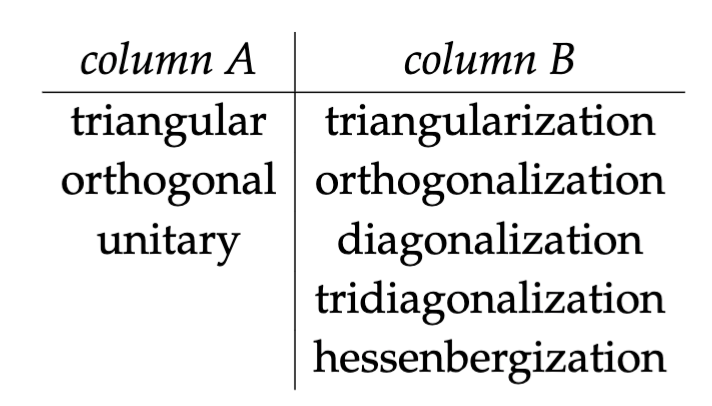
\includegraphics[width = .45\textwidth]{table.png}  
      \end{center}  
    \end{figure}
     \begin{enumerate}
      \item[a] Consider only the textbook Lectures which we covered, namely Lectures 1-17 and 20-27. For square matrices, 
      which distinct factorization do use, or easily could use, one of these 15 possible 2WPs? For each
       factorization, state the matrix factorization, its name and/or algorithm
        reference in the textbook, and it's 2WP.\\
      \solution  
      \begin{enumerate}
        \item[1] Gram-Schmidt ($A = QR$) (Triangular Orthogonalization)\\
        The Gram-Schmidt algorithm produces a QR factorization by repeatedly applying triangular matrices 
        to the right of $A$ to form an orthogonal matrix $Q$, as we saw in Lecture 8.
        \vspace{.15in}
        \item[2] Householder ($A = QR$) (Orthogonal Triagularization)\\
        The Householder Algorithm produces a QR factorization by repeatedly applying orthogonal matrices (Householder reflectors) the the left of $A$ 
        to form a triangular matrix, as we saw in Lecture 10.
        \vspace{.15in}
        \item[3] Gaussian Elimination ($A = LU$) (Triangular Triagularization)\\
        The Gaussian elimination algorithm produces an LU factorization by repeatedly applying lower triangular matrices (row operations) to the left of $A$ to 
        produce an upper triangular matrix, as we saw in Lecture 20. 
        \vspace{.15in}
        %%%%%%%%%%%%%%%%%%%%%%%%%%%%%%%%%%%%%%%%%%%%%%%%%%%%%%%%%%%%%% Look at this one again %%%%%%%%%%%%%%%%%%%%%%%%%%%%%%%%%%%%%%%%%%%%%%%%%%%%%%%%%%%%%%%%%%%%%%%%%%%%%%%%%%%%%%%%%%%%%%%%%%%
        \item[4] Cholesky ($A = R^*R$) (Triangular Triagularization)\\
        Cholesky factorization only succeeds when $A$ is a hermitian positive definite matrix, and it can be thought of as applying Gaussian Elimination on a symmetric matrix 
        with an extra factorization at each iteration which enables $L^*_i = U_i$. This factorization is described in detail in Lecture 23 and since it is a form of Gaussian Elimination 
        can be described as Triangular Triagularization
        %%%%%%%%%%%%%%%%%%%%%%%%%%%%%%%%%%%%%%%%%%%%%%%%%%%%%%%%%%%%%% Look at this one again %%%%%%%%%%%%%%%%%%%%%%%%%%%%%%%%%%%%%%%%%%%%%%%%%%%%%%%%%%%%%%%%%%%%%%%%%%%%%%%%%%%%%%%%%%%%%%%%%%%
        \vspace{.15in}
        \item[5] Shur Decomposition ($A = QTQ^*$) (Unitary Triagularization)\\
        The Shur Decomposition is obtained by applying unitary matrices constructed by normalized eigenvectors, as we saw in lecture 24 (Theorem 24.9).
        Interestingly since the Shur Decomposition is an eigenvalue revealing factorization, that is to say for matrices of a certain size it must be computed iteratively (as we did in one of the homework assignments).
        \vspace{.15in}
        \item[6] Unitary Diagonalization ($A = Q\Lambda Q^*$)\\
        Another eigenvalue revealing factorization, which can be thought of as Shur Decomposition when $A$ is a normal matrix, as we saw in Lecture 24. 
        \vspace{.15in}
        \item[7] Hessenberg Form ($A = QHQ^*$) (Unitary Hessenbergization)\\
         Hessenberg form is achieved by applying modified householder reflectors (leave the ith column/row unchanged) to the left and right sides of $A$, as we saw in lecture 26. 
        \vspace{.15in}
        \item[8] Tridiagonal Form ($A = Q\hat{T}Q^*$) (Unitary Tridiagonalization)\\
        Reduction to Tridiagonal Form is achieved when Hessenberg Algorithm is applied to a hermitian matrix $A$, as we saw in Lecture 26.
      \end{enumerate}
      \vspace{.25in}

    \item[b] The adjectives 'orthogonal' and 'unitary' are essentially synonyms. However the textbook systematically uses "unitary" for certain kind of factorization. 
    Explain, in a few sentences, the distinct purpose of the 'unitary' factorization.\\
    \solution The textbook defines an 'orthogonal' matrix as the real number equivalent to being unitary. To elaborate, when a matrix $A \in \CC^{mxm}$ has the property that $A^* = A^{-1}$ we say that 
    it is unitary, when a matrix $A \in \RR^{mxm}$ we can say it is orthogonal or unitary. The textbook makes sure to describe these matrices as 'unitary' when the factorization is an eigenvalue-revealing 
    factorization since 'even if the input to a matrix eigenvalue problem is real, the output may have to be complex.'(as stated in Theorem 24.1).
    \vspace{.25in}

    \item[c] The SVD factorization is not one of the answers in part (A). Why? Invent a good 2WP to describe it.\\
    \solution The SVD factorization reduces a matrix $A$ by $A = U\Sigma V^*$ where $U$ and $V$ are unitary, and $\Sigma$ is a diagonal matrix(with dimensions $A$). We can rewrite this factorization as 
    $U^*A V = \Sigma$ and then it can be thought of as Unitary Diagonalization. However when we computed the SVD we did so by solving the eigenvector, eigenvalue problem for $A^*A$ (or $AA^*$) and then used linear 
    systems to solve for leftover unitary factor, either $U$ or $V$ depending on how the problem was set up. I could see it being difficult to identify a two-word phrase that encapsulates that algorithm. \\
    \vspace{.25in}

    \item[d] Create, implement, and test an algorithm corresponding to a 2WP which is unused. that is invent an algorithm, which is not in the textbook and which is not listed in your part a answer.\\
    \solution Piggybacking off the last problem, since we have an algorithm which solves the eigenvalue problem, namely rqi we can link it together with Householder to produce the SVD.
     I think it would go like this, first we form $A^*A$, then we use Householder to find an orthogonal basis for $A^*A$ namely $Q$. Then we use the columns of $Q$ as initial guesses for rqi to solve the eigenvalue problem. We form 
     a unitary factor, then solve for the columns of the other by setting up the linear system and using householder.  
    \end{enumerate}

\end{exercise}

\newpage


\begin{exercise}{F2} 
  The producers and I believe we have a great new reality series, Naked and Calculating. (It will do great in the North Korean market \dots little competition.) The plan is to have three contestants,
  each seeking riches, on three islands. Each contestant will have unlimited supply of pencils and paper, plus adequate
  food and drink, but nothing else. Naturally, there are hidden cameras so we can watch the exciting action! Each island has a
  problem, and algorithm which the contestant must use:\\\\
  Island 1: Compute the determinant of an $mxm$ matrix using expansion in minors.\\
  Island 2: Solve an $mxm$ upper-triangular linear system using back-substitution.\\
  Island 3: Solve an $mxm$ linear system using Gaussian elimination.\\\\
  After finding-out which one is their island, a contestant chooses them value, but then the producers will choose generic
  values to fill the matrix entries.  By choosing m the contestants are gambling that they can compute the correct answer,
  by hand, in one month of work. In fact, at the end of one month a contestant either gets $2^m$ US dollars for correctly computing
  the solution of a problem, or zero dollars if their answer  is incorrect. (All entries in the final answer have to be correct to three digits.).\\
   \begin{enumerate}
     \item[a] As a contestant, which island would you choose? Most avoid? Please? Explain?\\
     \solution The choice between Island 2, and Island 3 is clear since solving a linear system using Gaussian Elimination requires us to reduce to an upper-triangular system, and then
     solve that by using back-substitution. Therefore, depending on $A$ Island 2 will always have less than or equal to the amount of work in Island 3. Recall that in Homework 2, Problem 6.b we computed that the number of FLOPs 
     for computing the determinant of an $mxm$ matrix was on the order of $O(m!)$ whereas the the text cites the number of FLOPs required for back substitution as $O(m^2)$ (17.2). As a contestant I would go for Island 2. 
    \vspace{.25in}


    \item[b] For each island, state the specific $m$ you would choose if you are put on that island. You must justify your choices via a quantitative, though necessarilly speculative, explaination.\\
    \solution As an estimate I think that typically I am able to perform an arithmetic operation once every 30 seconds. If I was doing this for real I would collect data for each operation and operation length, but for a rough estimate let's say
    one operation every 30 seconds. Computing an estimate for total operations in a 30 day period we get, 
    \begin{equation*}
      \dfrac{2 \text{ Operations}}{1 \text{ Minute}} \dfrac{60 \text{ Minute}}{1 \text{ Hour}} \dfrac{8 \text{ Hour}}{1 \text{ Day}}*30 = 28,800 \text{ Operations}
    \end{equation*}
    \begin{enumerate}
      \item[Island 1] Recall that the number of operations to compute the determinant of an $mxm$ matrix by expansion in minors is $O(m!)$. With a rough estimate of $28,800$ operations over the 30 day period I would have to choose $m = 7$, since 
      $7! = 5,040$ and $8! = 40,320$. This gives me a huge amount of time to double check my answers but it's unfortunate that increasing $m$ by one more has such a dramatic change in the number of operations.\\
      \item[Island 2] As was stated in the previous problem, the number of operations required to perform back substitution on a $mxm$ system is $\sim m^2$. With an estimate of $28,800$ operations over the 30 day period we get an $m$ value of 
      \begin{equation*}
        m = \sqrt{28800} \approx 169.7.
      \end{equation*} 
      So I would likely choose $m = 169$.\\
      \item[Island 3] The text states that the number of operations required to perform Gaussian elimination(no pivoting) on an $mxm$ system is $\sim \frac{2}{3}m^3$(20.8). With my estimate of $28,800$ operations over the 30 day period we get that, 
      \begin{equation*}
        m = (\dfrac{3}{2}28,800)^{\dfrac{1}{3}} \approx 35.08. 
      \end{equation*}
      So I would likely choose $m = 35$.\\
    \end{enumerate} 
    Clearly these are all upper bounds on $m$ as we would have to carve out time to double check computations. It is most definitely the case that using a single value is a poor way to model computations over time since there are various factors such as type of operation, number length, 
    and fatigue that should be taken into consideration. 
    \vspace{.25in}


    \item[c] For excitement, at the last minute before going on their island, after already having chosen an $m$ value, contestants are told that in fact they can choose their algorithm, and that they can 
    revise their $m$ choice. For one fo the islands this represents a huge improvement in the pay-out. Explain; give a new $m$ value with explanation.\\
    \solution Island 1 should compute their determinant by producing the $LU$ factorization of $A$. Note that if we let $A = LU$, then we get the following, 
    \begin{align*}
      det(A) &= det(LU),\\
      det(A) &= det(L)det(U),\\
      det(A) &= det(LU),\\
      det(A) &= \prod_{i = 1}^m U_{i, i}.
    \end{align*}
    This reduces the FLOPs to $ \sim \frac{2}{3}m^3 + (m-1)$, where we get $ \sim \frac{2}{3}m^2 $ operations to perform the $LU$ factorization and $(m-1)$ operations to evaluate the final product. Now that 
    Island 1 and Island 3 are using the same algorithm I would likely estimate the same $m = 35$ for Island 1 using this new method. I would note however that now Island 1 requires fewer operations than Island 3 since 
    after forming the $LU$ factorization all we need to do is evaluate the diagonal product $U$ which is order $m$ less expensive than performing back substitution.  
   \end{enumerate}
\end{exercise}
\newpage

\begin{exercise}{F3} Consider the following $A \in \RR^{3x4}$,
  \begin{equation*}
    A = \begin{bmatrix}
      2 &3 &5& -1\\
      -1& 7 &3 &5\\
      -1& -1& 2& 4
    \end{bmatrix}
  \end{equation*}
  Find the $B \in \RR^{3x4}$ of rank 2 which is the closest to $A$ in the 2-norm. \\
  \solution Recall from Theorem 5.7 that $A$ can be decomposed to a sum of $r$ rank-one matrices, where $r$ the rank of $A$, 
  \begin{equation*}
    A = \sum_{j = 1}^r \sigma_j u_j v^*_j.
  \end{equation*}
  Recall that by Theorem 5.8 the $v$ th partial sum, where $0 \leq v \leq r$ gives us the rank $v$, best approximation to $A$ under the 2-norm.
  The following Matlab script computes $B$, the second partial sum of $A$'s rank-one decomposition,\\
  \textbf{Code:}
  \begin{center}
  \lstinputlisting[basicstyle = \small]{F3.m}
  \end{center} 
\end{exercise}
\newpage




\begin{exercise}{F4} Expansion in minors may be a terrible algorithm for computing determinants, but it is backwards-stable. Prove this in the $1x1$ and $2x2$ 
  matrix cases, assuming as usual that your computer satisfies axioms (13.5) and (13.7).\\
  \solution Let $\tilde{f}$ be the Expansion in minors algorithm for the problem of computing the determinant of a matrix. Consider a $1x1$ matrix $A$ whose sole entry is $a_{11}$.
  We know that the determinant of a $1x1$ matrix is simply the single entry, so computing the algorithm $\tilde{f}(A)$, we get 
  \begin{equation*}
    \tilde{f}(A) = fl(a_{11}) = a_{11}(1 + \epsilon_1)= f(\tilde{A}).
  \end{equation*}
  Where $\tilde{A}$ is a $1x1$ matrix whose entry is $a_{11}(1 + \epsilon_1)$. By axiom (13.5) it follows that, 
  \begin{align*}
    \dfrac{||\tilde{A} - A||}{||A||} &= \dfrac{|a_{11}(1 + \epsilon_1) - a_{11}|}{|a_{11}|},\\
    &= \dfrac{|a_{11}((1 + \epsilon_1) - 1)|}{|a_{11}|},\\
    &= \dfrac{|a_{11}||\epsilon_1|}{|a_{11}|},\\
    &= \epsilon_1,\\
    &= O(\epsilon_{machine}).
  \end{align*}
  Thus the $1x1$ matrix case of Expansion in minors is backwards stable. \\\\
  Consider a $2x2$ matrix $A$ with the following entries,
  \begin{equation*}
    A  = \begin{bmatrix}
      a_{11} & a_{12}\\
      a_{21} & a_{22}
    \end{bmatrix}
  \end{equation*}
  Applying $\tilde{f}$ to $A$ we get the following, 
  \begin{align*}
    \tilde{f}(A) &= fl(a_{11})\otimes fl(a_{22}) \ominus fl(a_{21})\otimes fl(a_{12})\\
    &= (a_{11} a_{22})(1 + \epsilon_1) \ominus (a_{21} a_{12})(1 + \epsilon_2) \\
    &= ((a_{11} a_{22})(1 + \epsilon_1) - (a_{21} a_{12})(1 + \epsilon_2))(1 + \epsilon_3)\\
    &= (a_{11} a_{22})(1 + \epsilon_1)(1 + \epsilon_3) - (a_{21} a_{12})(1 + \epsilon_2)(1 + \epsilon_3)\\
    &= (a_{11}(1 + \epsilon_1)) (a_{22}(1 + \epsilon_3)) - (a_{21}(1 + \epsilon_2)) (a_{12})(1 + \epsilon_3))\\
    &=  (\tilde{a}_{11} \tilde{a}_{22})-(\tilde{a}_{21}\tilde{a}_{12})\\
    &= f(\tilde{A})
  \end{align*}
  Where $\tilde{A}$ is, 
  \begin{equation*}
    \tilde{A} = \begin{bmatrix}
      a_{11}(1 + \epsilon_1) & a_{12}(1 + \epsilon_3)\\
      a_{21}(1 + \epsilon_2) & a_{22}(1 + \epsilon_3)
    \end{bmatrix}.
  \end{equation*} 
  Now note that, 
  \begin{equation*}
    \tilde{A} - A = 
      \begin{bmatrix}
        a_{11}(1 + \epsilon_1) - a_{11} & a_{12}(1 + \epsilon_3) - a_{12}\\
        a_{21}(1 + \epsilon_2) - a_{21} & a_{22}(1 + \epsilon_3) - a_{22}
      \end{bmatrix}
      = 
      \begin{bmatrix}
        a_{11}\epsilon_1 & a_{12}\epsilon_3\\
        a_{21}\epsilon_2 & a_{22}\epsilon_3
      \end{bmatrix}
  \end{equation*}
  So applying the Frobenius norm we get the following, 
  \begin{align*}
    \dfrac{||\tilde{A} - A||_f}{||A||_f} &=  \dfrac{\left( (a_{11}\epsilon_1)^2 + (a_{12}\epsilon_3)^2 +(a_{21}\epsilon_2)^2 + (a_{22}\epsilon_3)^2 \right)^{\frac{1}{2}}}{   \left( (a_{11})^2 + (a_{12})^2 + (a_{21})^2 + (a_{22})^2 \right)^{\frac{1}{2}}},\\
    &\leq \dfrac{\left( (a_{11}\epsilon_{max})^2 + (a_{12}\epsilon_{max})^2 +(a_{21}\epsilon_{max})^2 + (a_{22}\epsilon_{max})^2 \right)^{\frac{1}{2}}}{   \left( (a_{11})^2 + (a_{12})^2 + (a_{21})^2 + (a_{22})^2 \right)^{\frac{1}{2}}},\\
    &= \dfrac{\left( a_{11}^2\epsilon_{max}^2 + a_{12}^2\epsilon_{max}^2 + a_{21}^2\epsilon_{max}^2 + a_{22}^2\epsilon_{max}^2 \right)^{\frac{1}{2}}} { \left( (a_{11})^2 + (a_{12})^2 + (a_{21})^2 + (a_{22})^2 \right)^{\frac{1}{2}}},\\
    &= \dfrac{\left((a_{11})^2 + (a_{12})^2 + (a_{21})^2 + (a_{22})^2 \right)^{\frac{1}{2}} \epsilon_{max}} { \left( (a_{11})^2 + (a_{12})^2 + (a_{21})^2 + (a_{22})^2 \right)^{\frac{1}{2}}},\\
    &= \epsilon_{max} = O(\epsilon_{machine}).
  \end{align*}
  Thus the $2x2$ matrix case of Expansion in minors is backwards stable.
\end{exercise}
\newpage


\begin{exercise}{F5} Recall the following ideas about our most trustworthy linear solver: Algorithm 10.1 is Householder triagularization $A = QR$. Code house.m implements this; read 
  and understand it! It outputs a lower triangular matrix $W$ containing the $v_k$ vectors and an upper triangular $R$, but of course $WR \neq A$. Next, Alg. 10.2 implements the action of $Q^*$
  from the vectors stored in $W$. Alg 16.1 adds back substitution (Alg.17.1) to give a solver for square, nonsingular linear systems $AX = b$. Theorem 16.2 shows that Alg. 16.1 is backwards-stable. \\
  Implement Alg16.1, but do it in-place. In particular, write a Matlab function,
  \begin{equation*}
    x = \text{inhousesolve(A,b)}
  \end{equation*}
  This function should start by checking that the inputs make sense i.e $A$ is square $(mxm)$ and b is a compatibly sized column vector. After that, the next line of your code should append one row of space to the bottom of the array $A$, like this, 
  \begin{equation*}
    A = [A; \text{zeros(1,m)}];
  \end{equation*}
  From now on, the only matrix or 2D array in your code is $A$ itself, and $A$ does not change size. You will modify entries of the array $A$, and the goal is to construct the vector $x$. 
  Inside your function you will implement Alg 10.1,  by modifying the entries of $A$ and to store $W$ and $R$, implement Alg 10.2 by referring to the entries of array $A$, and implement Alg 17.1 by referring to other entries of $A$.\\
  \solution Consider the following Matlab function,\\
  \textbf{Code:}
  \begin{center}
  \lstinputlisting[basicstyle = \small]{F5.m}
  \end{center} 
  \textbf{Console:}
  \begin{center}
  \lstinputlisting[basicstyle = \small]{F5Console.txt}
  \end{center} 
\end{exercise}
\newpage






\begin{exercise}{6}
  \begin{enumerate}
    \item[a] Implement Algorithm 26.1, Householder reduction to Hessenberg form, Specifically build code with the signature, 
    \begin{equation*}
      H = \text{hessen(A, stages)}
    \end{equation*} 
    Your code will check that $A$ is square, print the stages (next part) if stages is true, and finally return a Hessenberg matrix $H$ 
    such that $A = QHQ^*$ for some unitary $Q$. Note that your code can throw-away the vectors $v_k$; they are not returned. \\
    \solution Consider the following Matlab function,\\
    \textbf{Code:}
    \begin{center}
    \lstinputlisting[basicstyle = \small]{hessen.m}
    \end{center} 
    \vspace{.15in}


    \item[b] For a specific $5x5$ matrix $A$ of your choice, run the code and show the four stages 
    $A$, $Q^*_1AQ_1$,$Q^*_2Q^*_1AQ_1Q_2$, and $H = Q^*_3Q^*_2Q^*_1AQ_1Q_2Q_3$. That is, make concrete the cartoons on pages 197-198, 
    'A Good Idea'. \\
    \solution Calling hessen() on a $5 x 5$ magic matrix $A$ we get,\\ 
    \textbf{Console:}
    \begin{center}
    \lstinputlisting[basicstyle = \small]{F6b.txt}
    \end{center} 
    \vspace{.15in}

    \item[c] For the same $5x5$ matrix $A$, use the built-in eig() to show that the eigenvalues of $A$ and $H$ are the same within rounding error. 
    Now construct a new $4x4$ hermitian matrix $S$ and compute $T = hessen(S)$. Check that $T$ is tridiagonal and Hermitian. Then show the eigenvalues of $S$ 
    and $T$ are the same within rounding error. \\
    \solution Generating the eig values of $A$ and $H$ using the built-in eig() we find that they are within rounding error, with the 2-norm of the difference having size on the 
    order of $10^{-14}$.\\
    \textbf{Console:}
    \begin{center}
    \lstinputlisting[basicstyle = \small]{F6c1.txt}
    \end{center} 
    Computing a $4x4$ hermitian matrix $S$ and computing it's tridiagonal decomposition $T$ we get that the eigenvalues, when computed with the built-in eig() function are within rounding error on the order of 
    $10^{-12}$.\\
    \textbf{Console:}
    \begin{center}
    \lstinputlisting[basicstyle = \small]{F6c2.txt}
    \end{center}  
  \end{enumerate}
\end{exercise}
\newpage



\begin{exercise}{F7} Implement Algorithm 27.3, namely Rayleigh quotient iteration. In particular, write a Matlab code with the signature:
  \begin{equation*}
    [lam, v] = \text{rqi(A, v0)}
  \end{equation*}
  which returns an eigenvalue $lam$ corresponding to the eigenvector $v$, and which starts the iteration with $v0$. You will need a stopping criterion to avoid 
  a warning when solving the linear system with the matrix $B = A = \lambda^{k - 1}I$. I suggest stopping when,
  \begin{equation*}
    rcond(B) < 10*eps
  \end{equation*}
  (Using Matlab documentation, explain what this criterion means.) Show your code works by $(i)$ reproduce the iterates $\lambda^{0}$, $\lambda^{1}$, $\lambda^{2}$ in 
  Example 27.1, and $(ii)$ by matching one of the eigenvalues and eigenvectors of a random $20x20$ Hermitian matrix. (For $(ii)$, assume that the built in eig() is exact.)\\
  \solution Consider the following Matlab function, \\
  \textbf{Code:}
    \begin{center}
    \lstinputlisting[basicstyle = \small]{rqi.m}
    \end{center} 

  \begin{enumerate}
    \item[i] Reproducing the iterates from example 27.1 we get the following, \\
    \textbf{Console:}
    \begin{center}
    \lstinputlisting[basicstyle = \small]{F7i.txt}
    \end{center} 
    \vspace{.15in}

    \item[ii] Matching a rqi() computed eigenvector, eigenvalue pair from a random $20x20$ hermitian 
    matrix with eig() we get, \\
    \textbf{Console:}
    \begin{center}
    \lstinputlisting[basicstyle = \small]{F7ii.txt}
    \end{center} 
    \vspace{.15in}

     
  \end{enumerate}
  

\end{exercise}





\end{document}




















